\documentclass[10pt,letterpaper,twocolumn]{article}

%2012-10-01 - Document préparé par David Lafrenière, pour le cours PHY3040.

%Pour langue et caractères spéciaux
\usepackage[french]{babel} 
\usepackage[T1]{fontenc}
\usepackage{lmodern}
\usepackage[utf8]{inputenc}

\usepackage[backend=biber, style=nature]{biblatex}
\addbibresource{reference.bib}


%Package for math expression
\usepackage{amsmath}
\usepackage{amsthm,amstext,amsfonts,bm,amssymb,amsthm}
\usepackage{mathtools}
\usepackage{bm}
\usepackage{gensymb}
\usepackage{mathrsfs}
\usepackage{physics}

%Package for drawings
\usepackage{tikz}
\usepackage{pgfplots}% loads also tikz
\pgfplotsset{compat=newest}% to avoid the pgfplots warning
\usetikzlibrary{intersections, pgfplots.fillbetween}
\usetikzlibrary{calc,patterns,angles,quotes}
\usepackage[compat=1.1.0]{tikz-feynman}
\usetikzlibrary{3d}
\usetikzlibrary{decorations.pathreplacing}
\usepackage{lineno}

%Package pour les symbole astronomiques
%\usepackage{wasysym}

\usepackage{hyperref}

%Pour ajuster les marges
\usepackage[top=2cm, bottom=2cm, left=2cm, right=2cm, columnsep=20pt]{geometry}

% Pour la commande onecolabstract (résumé 1 pleine largeur)
\usepackage{abstract}
	\renewcommand{\abstractnamefont}{\normalfont\bfseries}
	\renewcommand{\abstracttextfont}{\normalfont\itshape}

% Pour les titres de section/sous-section
\usepackage[compact]{titlesec}
\titleformat{\section}{\large\bfseries}{\thesection}{1em}{}
\titleformat{\subsection}{\normalsize\bfseries}{\thesubsection}{1em}{}
\titleformat{\subsubsection}{\normalsize}{\thesubsubsection}{1em}{}

%Package for graphic expression
\usepackage{graphicx}
\usepackage{wrapfig}
\usepackage{float}
\usepackage{caption}
\usepackage{subcaption}
\usepackage{enumitem}

%Shorthand for space and some math expressions
\newcommand{\s}{\hspace{0.1cm}}
\renewcommand{\Im}{\operatorname{\mathbb{I}m}}
\renewcommand{\Re}{\operatorname{\mathbb{R}}}
%Shorthand for partial differential
\newcommand{\partialD}[2]{\frac{\partial #1}{\partial #2}}
%Shorthand for \left(\right)
\DeclarePairedDelimiter\autobracket{(}{)}
\newcommand{\br}[1]{\autobracket*{#1}}

\newcommand{\pyoutput}[2]{#2} % Simply output #2, use #1 as tag for python reader

%pour tableaux deluxetable
%\usepackage{deluxetable}

%Pour inclure des adresse web
\usepackage{url}

%Titre
\title{\vspace{-10mm}\Large
Faisceaux gaussiens %%%***éditer cette ligne***
\vspace{-4mm}}

%Auteur
\author{\large
Alexandre Adam
}
\date{\vspace{-8mm}}
\captionsetup{labelfont=bf, format=plain, font=footnotesize}
\begin{document}

\twocolumn[
\maketitle
\begin{onecolabstract} % 10 points
Les paramètres de propagations $z_0$, $w_0$, $\mathcal{I}m\left\{q_0\right\}$ et $\theta_0$ sont estimés expérimentalement et comparés avec les paramètres de propagation prédits par l'optique matricielle dans l'approximation des lentilles minces. On trouve que l'accord varie entre $4\%$ et $15\%$, pour un paramètre à la fois, exhibant les effets d'optimisation du <<no free lunch theorem>>. On observe la demie-largeur $w_0 = (101 \pm 2) \s \mu\text{m}$ pour une lentille avec $f = 17.5\s \text{mm}$, une taille caractéristique $4\%$ plut petite que la largeur attendue $w_0 = (105.6 \pm 0.1) \s \mu\text{m}$. On observe aussi qu'un système moins convergent atteint systématiquement une demie-largeur plus grande que la valeur prédite ($8\%$ et $15\%$), alors que la précision sur $z_0$ s'améliore pour des systèmes moins convergents ($8\%$ puis $4\%$). 
\vspace{4mm} %
\end{onecolabstract}
]

\section{Introduction}\label{intro} % 5 points
La concentration d'un faisceau gaussien dans un système optique prend une place importante dans plusieurs applications techniques, ainsi que dans le recherche. Pour ne nommer que l'exemple le plus important, la pince optique (\textit{optical tweezers}) permet de manipuler des particules ou des cellules organiques en les capturant au point où le faisceau gaussien atteint son minimum ($z_0$). Cette application a valu le prix Nobel à Arthur Ashkin en 2018, et fût à la base des travaux de Claude Cohen-Tannoudji, Steven Chu et William Philips qui ont reçu le prix Nobel en 1997 pour leur travaux sur le refroidissement et le piégeage d'atomes. \par
Dans ces applications, la prédiction précise des paramètres de propagation $w_0$ et $z_0$ est d'une importance cruciale. On investigue, dans cette expérience, les prédictions de l'optique matricielle paraxiale avec l'approximation des lentilles minces, dont le développement théorique est dû à Stuart A. Collins\supercite{Collins1970} (1970).\par
En premier lieu, on extrapole le paramètre de taille complexe à l'extrémité du laser, puis on utilise ce paramètre pour prédire la position du minimum pour des systèmes optiques de 1, 2 et 3 lentilles. On choisit les systèmes telles que leur longueur focale équivalente augmente de façon croissante pour déterminer l'effet de la convergence du faisceau sur les paramètres de propagation.

\section{Théorie}\label{sec:theorie} % 10 points
Un faisceau gaussien est décrit par le champ électrique\supercite{Pedrotti}
\begin{align}
\nonumber	\tilde{E} = &E_0\exp\bigg\{\frac{w_0}{w(z)}-\rho^2/w^2(z)+ik\rho^2/2R(z) \\
									&\hspace{0.2cm}-i\arctan(z/z_0)+i(kz - \omega t + \phi)\bigg\}.
\end{align}
Ce champ électrique est solution des équations de Maxwell dans l'approximation paraxiale, avec une symétrie cylindrique autour de l'axe optique $z$. $\rho$ est le rayon cylindrique. On définit le paramètre de demie-largeur
\begin{equation}\label{eq:w}
	w^2(z, w_0, z_0) = w_0^2\br{1 + \frac{(z - z_0)^2}{z_R^2}}
\end{equation}
qui atteint son minimum à $z_0$, là où le paramètre de taille complexe $q(z)$ est purement imaginaire:
\begin{equation}\label{eq:q}
	\frac{1}{q(z)} = \frac{1}{R(z)} + i\frac{\lambda}{\pi w^2(z)}.
\end{equation}
$z_R$, la longueur de Rayleigh est définit comme
\begin{equation}
	z_R = \frac{\pi w_0^2}{\lambda}.
\end{equation}
$w_0$ est la largeur minimal du faisceau. \par
La propagation du faisceau dans un système optique est décrite à l'aide des éléments de la matrice ABCD de l'optique géométrique. Le paramètre de taille complexe sur le plan image est donné par\supercite{Collins1970}
\begin{equation}\label{eq:ABCD}
	\frac{1}{q(z_2)} = \frac{C + D/q(z_1)}{A + B/q(z_1)}.
\end{equation}
Les paramètres A, B, C et D sont déterminées par la composition de la matrice de transfert 
\begin{equation}
	\mathbf{T} = \left[\begin{matrix}
		1 & d\\
		0 & 1
	\end{matrix}    \right]
\end{equation}
et la matrice pour des lentilles minces
\begin{equation}
	\mathbf{R} = \left[ \begin{matrix}
		1 & 0 \\
		-\dfrac{1}{f} & 1
	\end{matrix}   \right]
\end{equation}
du point $z_1$ à $z_2$.\par
On définit finalement l'angle de divergence $\theta$: lorsque $z \gg z_R$, la largeur du faisceau augmente linéairement avec la distance
\begin{equation}\label{eq:theta}
	w(z\gg z_R) \approx \theta_0 z,\hspace{0.2cm} \theta_0 = \frac{\lambda }{\pi w_0}
\end{equation}
\par



\section{Méthodologie}\label{sec:metho} % 15 points
Le montage utilisé comporte une source laser He-Ne produisant un faisceau monochromatique de longueur d'onde $\lambda = 632.8\s \text{nm}$. On analyse la propagation de ce faisceau avec un système optique pouvant comporter jusqu'à trois lentilles. \par
Les mesures des paramètres $w_0$ et $z_0$ se fait indirectement à partir de la mesure de l'intensité lorsque le faisceau est coupé par une lame de rasoir se déplaçant selon l'axe $x$ (voir Figure \ref{fig:montage}). L'intensité est mesurée à l'aide d'un picoampèremètre. En prenant un profil d'intensité selon $x$, on est en mesure d'estimer les paramètres locaux de propagation. 
\begin{figure}[H]
	\centering
	\resizebox{\linewidth}{!}{
	\begin{tikzpicture}
	\draw (-0.5, 0.5) rectangle (1, -0.5) node[pos=.5] {Laser};
	\node at (0, -1	) {$\lambda = 6328\s \text{\AA}$};
	\draw[color=red, name path=A] (1, 0.3) .. controls (2, 0.6) and (4, -0.2) ..(6, 0.3);
	\draw[color=red, name path=B]  (1, -0.3) .. controls (2, -0.5) and (4, 0.2) .. (6, -0.3);
	\tikzfillbetween[of=A and B]{red, opacity=0.1};
	\begin{scope}[canvas is zy plane at x=1.7]
		\pgfmathsetmacro{\lensRadius}{1.5}
		\pgfmathsetmacro{\lensHeight}{1}
		\pgfmathsetmacro{\startAngle}{asin(\lensHeight/\lensRadius)}
		  \draw[name path=C] (0,\lensHeight) arc[start angle=180-\startAngle,delta angle=2*\startAngle,radius=\lensRadius];
		  \draw[name path=D] (0,\lensHeight) arc[start angle=\startAngle,delta angle=-2*\startAngle,radius=\lensRadius];
		  \tikzfillbetween[of=C and D]{gray, opacity=0.1};
	\end{scope}
	\node at (2.3, -1.3) {Lentille(s)};
	\draw[<->] (1, -2) -- (6, -2);
	\node at (3.5, -2.3) {$z$};
	\begin{scope}[canvas is yz plane at x=6]
	    \filldraw[even odd rule, inner color=red, outer color=white] (0,0) circle (0.3);
		\draw (-0.75,0.75) rectangle (0.75,-0.75);
	\end{scope}
	\begin{scope}[canvas is yz plane at x=5.6]
		\filldraw[color=gray, opacity=0.8] (-0.75,0.3) rectangle (0.75,1);
	\end{scope}
	
	\begin{scope}[canvas is yz plane at x=5.5]
		\draw[->] (-1, 1) -- (-1, 0);
		\node at (-1.2, 1) {$x$};
	\end{scope}
	\node at (6.5, -1.5) {Photodiode};
	\draw (6, 0.75) ..controls (6.5, 0.2) .. (7,0.5);
	\draw (7, 0.5) rectangle (10, -0.5) node[pos=.5] {Picoampèremètre};
	\node at (5, 1) {Lame};
	\end{tikzpicture}
	}
	\caption{Montage de l'expérience. Un laser He-Ne produit un faisceau qu'on fait passer au travers d'un système optique, comportant 0/1/2/3 lentilles. L'intensité est mesuré à l'aide d'une photodiode et lue à l'aide du picoampèremètre. La lame se déplace à l'aide d'une vis micrométrique.}
	\label{fig:montage}
\end{figure}


\subsection{Estimation de la $w(z)$}\label{sec:wz}
La lame de rasoir de la figure \ref{fig:montage} balaye la direction $x$, perpendiculaire à l'axe optique, pour soustraire une partie de l'intensité du faisceau gaussien. Cette portion est proportionnelle à la fonction d'erreur\supercite{Yoshida1976} et la courbe de l'intensité en fonction de la position de la lame est de la forme
\begin{equation}\label{eq:I}
	I_z(x) = \frac{I_0}{2}\br{1 - \erf\left[\frac{\sqrt{2}(x-x_0)}{w(z)}  \right]  },
\end{equation}
où $x_0$ est la position où l'intensité est maximale. On obtient le paramètre $w(z)$ avec un ajustement par moindres carrés de la courbe $I_z(x)$. On répète cette procédure en balayant l'axe optique $z$ avec la photodiode pour obtenir le profil $w(z)$. Un ajustement de l'équation \eqref{eq:w} sur ce profil permet finalement d'estimer les paramètres $w_0$ et $z_0$.\par
Ces valeurs sont ensuite comparés aux valeurs prédites par l'équation \eqref{eq:ABCD}, qu'on projette à partir de $q(z=0)$, soit l'extrémité du laser.

%\subsection{Estimation des paramètres ABCD}
%L'équation \eqref{eq:ABCD} permet d'estimer les paramètres A, B, C, et D pour les comparer avec les éléments de la matrice du système optique qu'on obtient en appliquant les règles de l'optique géométrique paraxiale. Pour ce faire, on estime d'abord $q(z_1)$ en mesurant les paramètres $w_0$ et $z_0$ de la propagation sans lentille.
% $q(z_2)$ se situe dans le plan image du système optique. On choisit donc des systèmes optiques qui produisent une image réelle est suffisamment éloignée des lentilles pour que nos mesures puissent déterminer directement la position du minimum de la demie-largeur du faisceau.

% Dans cette expérience, on considère des lentilles minces (avec une distance focale $>150\s \text{mm}$)


\section{Résultats et discussion}\label{sec:resultats} % 25 points
\subsection{Sans lentilles}
L'expérience sans lentilles permet d'estimer le paramètre $q(z_0)$ qui est utilisé pour propager les faisceaux avec l'équation \eqref{eq:ABCD}. La figure \ref{fig:fit} montre trois ajustements de l'équation \eqref{eq:I} sur les données prises en laboratoire. Le paramètre $w(z)$ est obtenu directement à partir de l'ajustement par les moindres carrés, mais peut aussi être obtenu à partir des donnés de la figure \ref{fig:fit} en considérant que $1.28w(z) \approx x(I = 0.1I_{max}) - x(I = 0.9I_{max})$.


\begin{figure}[H]	
\centering
\begin{subfigure}[t]{0.45\linewidth}
	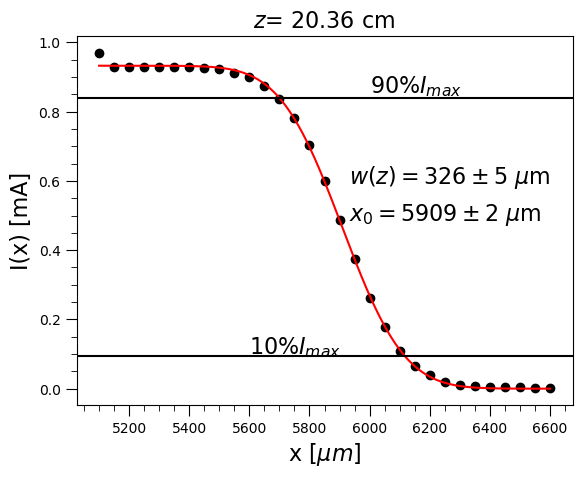
\includegraphics[width=\linewidth]{figures/0_2036_fit.png}
\end{subfigure}
\begin{subfigure}[t]{0.45\linewidth}
	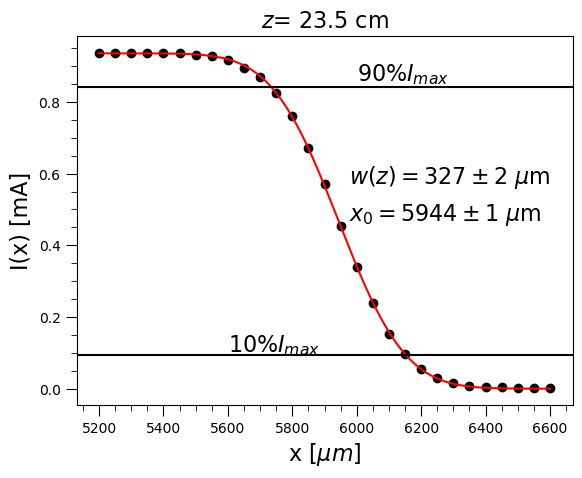
\includegraphics[width=\linewidth]{figures/0_2350_fit.png}
\end{subfigure}
~
\begin{subfigure}[t]{0.6\linewidth}
	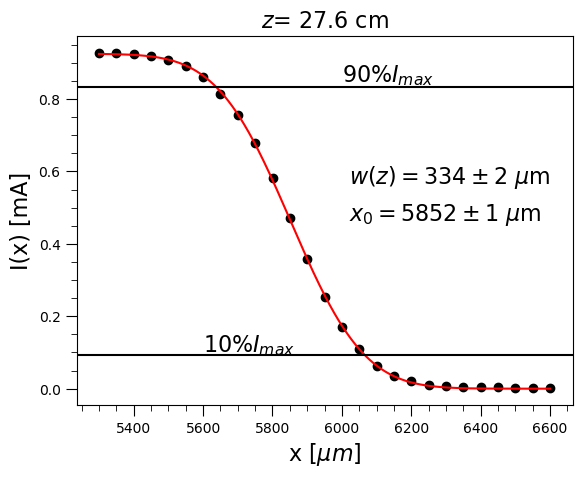
\includegraphics[width=\linewidth]{figures/0_2760_fit.png}
\end{subfigure}

\caption{Données d'intensités mesurées par le picoampèremètre (voir montage, figure \ref{fig:montage}) en fonction de la position de la lame. $x_0$ représente la position du centre du faisceau gaussien. }
\label{fig:fit}
\end{figure}

On remarque que $x_0$ varie légèrement dans les différentes figures. Cette différence est dû à l'alignement optique; l'angle par rapport $x$ est ajusté au début de l'expérience pour être le plus petit possible, mais une valeur non-nulle cause des déplacements de quelques micromètres dans la direction $x$ lorsqu'on recule le détecteur, suggérant que le système est mal aligné. Ceci peut amplifier les effets d'aberration coma en particulier, et causer un déplacement du minimum $z_0$ sur l'axe optique. 

\begin{figure}[H]
\centering
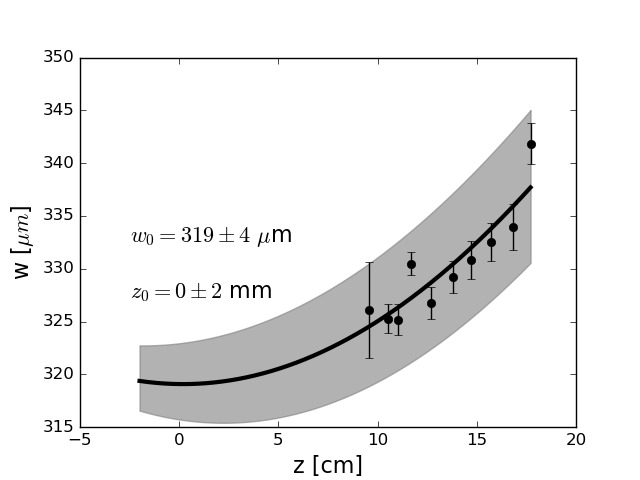
\includegraphics[width=\linewidth]{figures/w1.png}
\caption{Paramètres de propagations $w_0$ et $z_0$ extrapolés à partir des données récoltés dans le champ image de la source laser He-Ne. L'extrapolation est particulièrement mauvaise pour l'estimation de $z_0$, qui se trouve autour de l'extrémité du laser. }
\label{fig:w1}
\end{figure}


\subsection{1 lentille}
On place une lentille de longueur focale $f=175\s \text{mm}$ à une distance de $33.1\s {cm}$ du laser. On estime la largeur du faisceau par la méthode décrite à la section \ref{sec:wz}. La figure \ref{fig:w2} montre les résultats de l'expérience, ainsi que la courbe obtenu par la propagation paraxiale de $q(z=0)$ par l'équation \eqref{eq:ABCD} (ligne pointillée). 
\begin{figure}[H]
	\centering
	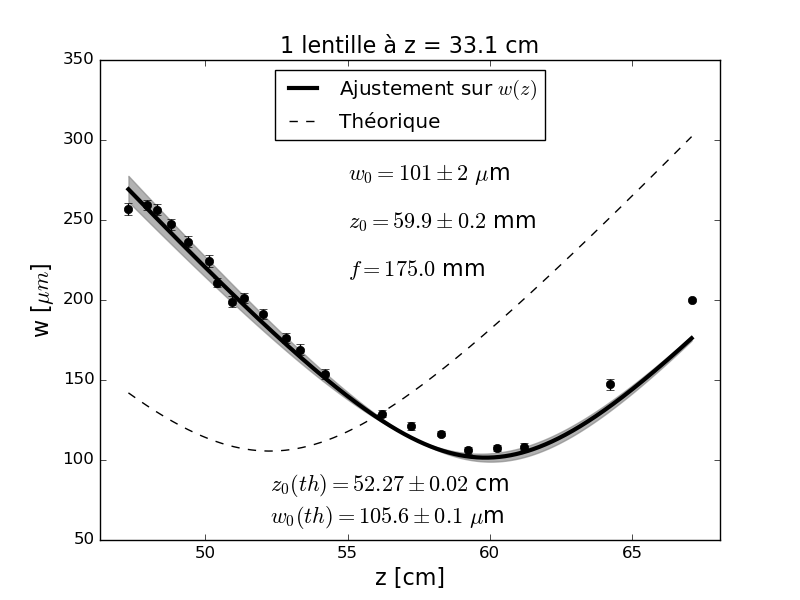
\includegraphics[width=\linewidth]{figures/w2.png}
	\caption{Comparaison entre la prédiction du profil de largeur du faisceau par l'équation \eqref{eq:ABCD} (théorie) et l'ajustement expérimental des paramètres $w_0$ et $z_0$ de l'équation \eqref{eq:w}. }
	\label{fig:w2}
\end{figure}
La table \ref{tab:w2} compare l'estimation des paramètres de propagation $w_0$, $z_0$, $q_0$ et $\theta_0$ expérimentaux avec les paramètres extrapolés de la mesure de $w_0$ par l'expérience sans lentille et l'application de l'équation \eqref{eq:ABCD}. 
\begin{table}[H]
	\centering
	\caption{Paramètres de propagation pour 1 lentille}
	\label{tab:w2}
	\begin{tabular}{|c|c|c|}
		\hline
			&Expérimental & Théorique \\\hline
		  $w_0$ [$\mu$m] & $101 \pm 2$& $105.6 \pm 0.1$ \\\hline
		  $z_0$ [cm] & $59.9 \pm 0.2$  & $52.27 \pm 0.02$ \\\hline
		  $\mathcal{I}m\{q_0\}$ [cm]  & $5.1 \pm 0.1$  & $5.534 \pm 0.005$ \\\hline
		  $\theta_0$ [arcmin]& $6.8 \pm 0.2$ & $6.558 \pm 0.006$ \\\hline
	\end{tabular}
\end{table}
La Table \ref{tab:w2}) montre que la demi-largeur minimale est en accord avec l'expérience, mais le faisceau atteint son minimum $z_0$ quelques centimètres plus loin que prévu.
Pour un faisceau gaussien, le minimum tend à se situer près du point focal $z_2 \approx f$ lorsque $w_{01} \gg w_{02}$, mais en général\supercite{Pedrotti}
\begin{equation}
	z_2 = f + \frac{f^2(z_1 - f)}{(z_1 - f)^2 + (\pi w_{01}^2 / \lambda)^2}
\end{equation}
Le faisceau ne se concentre pas au point focal pour des lentilles suffisamment convergentes. Cette différence est de l'ordre de $1.6\s \text{cm}$ théoriquement, et ne peut expliquer la déviation de $9.3\s \text{cm}$ expérimentale. 

\subsection{2 lentilles}
Deux lentilles avec $f_1=1000\s \text{mm}$ et $f_2 = 500\s \text{mm}$ sont placées à $z=29.2\s \text{cm}$ et $z = 36.2\s \text{cm}$ respectivement de la source laser. Le choix des longueurs focales est motivé par la recherche d'un point $z_2$ où le faisceau se concentre dans la plan image du système optique, de telles sortes que nos instruments puissent le mesurer directement. Or, en général, les systèmes à deux lentilles très convergente produisent une image qui tend à se situer du côté virtuel (microscopes), ce qui se montre facilement à partir de la longueur focale équivalente du système:
\begin{equation}
	F = \frac{f_1f_2}{f_1 + f_2 - d}
\end{equation}
où $d$ est l'espace entre les lentilles. Nous avons utilisé l'estimation très approximative $z_2 \approx F = 34.9\s \text{cm}$ pour choisir les lentilles qui nous permettraient d'obtenir $z_2$ dans le plan image à une distance suffisante du système optique pour que $w_0$ puisse être observé directement. \par
La figure \ref{fig:w3} montre les résultats de l'expérience.

\begin{figure}[H]
	\centering
	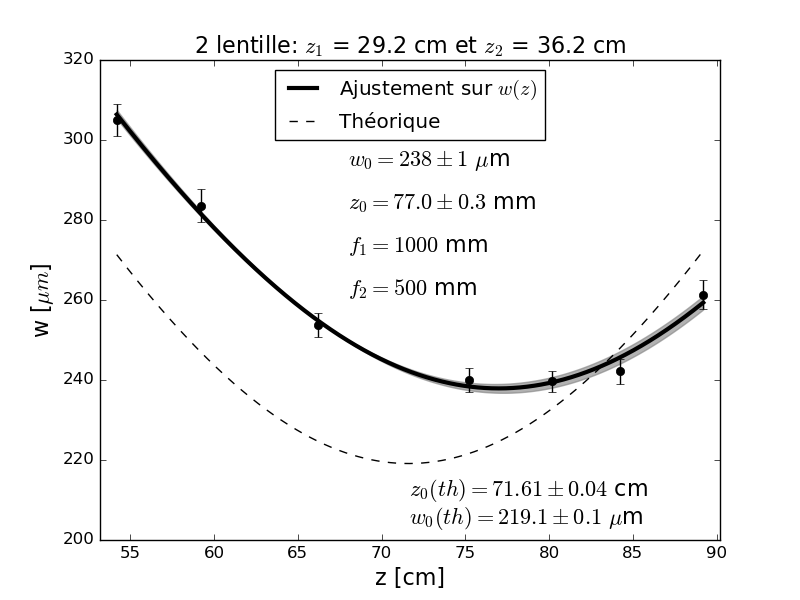
\includegraphics[width=\linewidth]{figures/w3.png}
	\caption{Comparaison de la demi-largeur théorique, propagée à partir de $q(z=0)$, et la demi-largeur expérimentale. Les paramètres $w_0$ et $z_0$ observés diffèrent de façon très importante pour cette expérience. }
	\label{fig:w3}
	
\end{figure}
 On observe encore une fois une différence au niveau de la position de minimum (Table \ref{tab:w3}), mais on observe aussi que le faisceau n'atteint pas la taille minimale prédite par la théorie, contrairement au système à une lentille. Il est à noter que la différence entre la position du minimum théorique et expérimentale s'est légèrement réduite en comparant aux système à une lentille plus convergent. Cette tendance se poursuit de façon marquée pour un système à trois lentilles qui converge encore plus lentement que ce système. \par La Table \ref{tab:w3} résume les paramètres de propagation du faisceau.
\begin{table}[H]
	\centering
	\caption{Paramètres de propagation pour 2 lentilles}
	\label{tab:w3}
	\begin{tabular}{|c|c|c|}
		\hline
			&Expérimental & Théorique \\\hline
		$w_0$ [$\mu$m] & $238 \pm 1$& $219.1 \pm 0.1$ \\\hline
		  $z_0$ [cm] & $77.0 \pm 0.3$  & $71.61 \pm 0.04$ \\\hline
		  $\mathcal{I}m\{q_0\}$ [cm]  & $28.0 \pm 0.1$  & $23.84 \pm 0.01$ \\\hline
		  $\theta_0$ [arcsec]& $174.6 \pm 0.8$ & $189.611 \pm  0.001$ \\\hline
	\end{tabular}
\end{table}

\subsection{3 lentilles}
Pour ce système, il était encore important d'utiliser l'estimation de la distance focal équivalente pour déterminer un système optique à trois lentille qui puisse converger dans le plan image. On utilise une lentille divergente pour agrandir le faisceau, avec ${f_2 = -250\s \text{mm}}$, placée entre une lentille lentement convergent ${f_1 = 1000\s \text{mm}}$ et une deuxième lentille bi-convexe ${f_3 = 250\s \text{mm}}$. On obtient $F \approx 55.5\s \text{cm}$, ce qui se trouve à $z_2 = 94.7\s \text{cm}$. Le résultat de l'expérience est dépicté dans la Figure \ref{fig:w4}.
\begin{figure}[H]
	\centering
	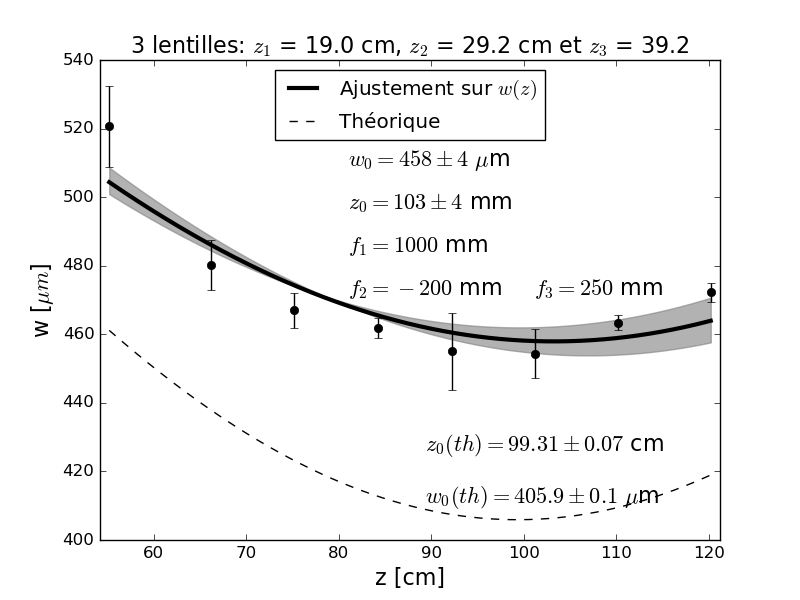
\includegraphics[width=\linewidth]{figures/w4.png}
	\caption{}
	\label{fig:w4}
\end{figure}
Les mesures de $z_0$ théorique et expérimentales ont maintenant une différence de $4\%$, contrairement à $8\%$ pour le système à deux lentilles et $13\%$ pour le système à une lentille. Alors qu'on a améliorer l'accord théorique pour la position du minimum $z_0$, la demie-largeur minimale $w_0$ est maintenant $15\%$ plus grande que la valeur attendue, contrairement à $8\%$ pour 2 lentilles et $-4\%$ (plus petite) pour 1 lentille. L'optimisation apportée par un système moins convergent pour prédire la position de $z_0$ exhibe les caractéristiques du \textit{no free lunch theorem}; en améliorant la prédiction d'un paramètre on perd de la précision sur l'autre.\par
Les paramètres de propagations sont listés dans la Table \ref{tab:w4}.


\begin{table}[H]
	\centering
	\caption{Paramètres de propagation pour 3 lentilles}
	\label{tab:w4}
	\begin{tabular}{|c|c|c|}
		\hline
			&Expérimental & Théorique \\\hline
		$w_0$ [$\mu$m] & $458 \pm 4$& $405.9 \pm 0.1$ \\\hline
		  $z_0$ [cm] & $103.4 \pm 0.3$  & $99.31 \pm 0.07$ \\\hline
		  $\mathcal{I}m\{q_0\}$ [cm]  & $104.1 \pm 0.9$  & $81.80 \pm 0.02$ \\\hline
		  $\theta_0$ [arcsec]& $90.7 \pm 0.8$ & $102.3531 \pm  0.0001$ \\\hline
	\end{tabular}
\end{table}

Les angles de divergence du faisceaux, compilés aux Tables \ref{tab:w2}, \ref{tab:w3} et \ref{tab:w4} sont suffisamment petits pour justifier l'utilisation de l'approximation paraxiale sous-entendue dans l'utilisation de l'optique matricielle. Ainsi, pour expliquer les disparités observés pour les paramètres $w_0$ et $z_0$, on peut se tourner vers les aberrations optiques. En particulier, l'aberration sphérique peut contribuer à déplacer $z_0$ sur l'axe optique de façon proportionnel à $r^2$\supercite{Pedrotti}, où $r$ est le diamètre de la surface réfractante. Or, cette aberration peut causer une étendue du point focal de l'ordre d'un dixième de centimètre, soit un ordre de grandeur plus petit que les disparités observées. 

\section{Conclusion}\label{sec:conclusion} % 10 points
La prédiction des paramètres de propagations par la méthode de l'optique matricielle, avec l'approximation des lentilles minces, ne permet d'atteindre une précision inférieur à $5\%$ qu'avec un paramètre à la fois. En utilisant un système avec une longueur focale suffisamment courte ($f < 200\s \text{mm}$), le faisceau est réduit à une taille $w_0 = (101 \pm 2) \s \mu\text{m}$, soit $4\%$ plus petit que la taille prédite par la théorie. Toutefois, la précision sur $z_0$ est à son maximum pour se système ($13\%$), et le système converge $7.6\s \text{cm}$ plus loin que prévu. En utilisant plusieurs lentilles et en réduisant la convergence du système, on améliore la précision sur $z_0$ jusqu'à $4\%$, mais le faisceau n'atteint plus la taille minimale théorique et on perd jusqu'à $15\%$ de précision sur l'estimation de $w_0$.\par
Les disparités observés dans ce laboratoire suggèrent qu'une investigation plus approfondie des approximations des lentilles pourrait permettre d'éclaircir les disparités observées dans les résultats. De plus, l'analyse conduite dans cette expérience suppose la présence d'un seul mode, soit $TE_{00}$. La présence de modes secondaires pourrait causer des déviations au comportement attendu, et possiblement expliquer les disparités observées. 



\printbibliography



\end{document}
